\begin{table}[htbp]
\centering\small
\begin{tabularx}{\textwidth}{p{10mm}Xccc}
\toprule
Job & Fresh consumer scope and transition & A & B & C2\\
\midrule
F01 & Flask startup banner; Click 8.1.7 to 8.2.1 & Pass & Pass & Pass\\
F02 & Black output/error formatting; same Click transition & Pass & Pass & Pass\\
F03 & NetworkX eigenvector centrality; SciPy 1.10.1 to 1.14.1 & Pass & Pass & Fail\\
F04 & Hugging Face Hub HTTP client factories; HTTPX 0.27.2 to 0.28.1 & Pass & Pass & Pass\\
\bottomrule
\end{tabularx}
\caption{Frozen customer-report acceptance on four new historical work packages. ``Pass'' is bounded internal acceptance, not observed buyer acceptance, runtime compatibility or approval to upgrade.}
\end{table}

All twelve scheduled follow-up executions completed once. A and B pass all four frozen customer-report checks; C2 passes three. The independent inventory contains twelve required calls: six conditional preserved bindings and six required unresolved calls. All three arms agree on those required conclusions. There are no material omissions, wrong selected targets or unsupported production approvals. B does not improve accepted quality over A.

C2 adds two spurious operations in F03: \texttt{eigenvector.flatten()} and \texttt{largest.sum()}. The prefreeze oracle explicitly excludes these NumPy/data operations from the SciPy-call inventory. The captured SciPy \texttt{eigs} return documentation identifies its eigenvectors as ndarray values, and the captured NetworkX code operates on that returned value. This is a source-contract argument under ordinary imports, not a measured runtime-type assertion. C2's error is over-inclusion; it is not an unsafe upgrade approval or a wrong binding result. In F02, C2's refusal to decide expanded \texttt{**styles} calls is justified and agrees in substance with the core's unresolved A/B result.

\begin{figure}[htbp]
\centering
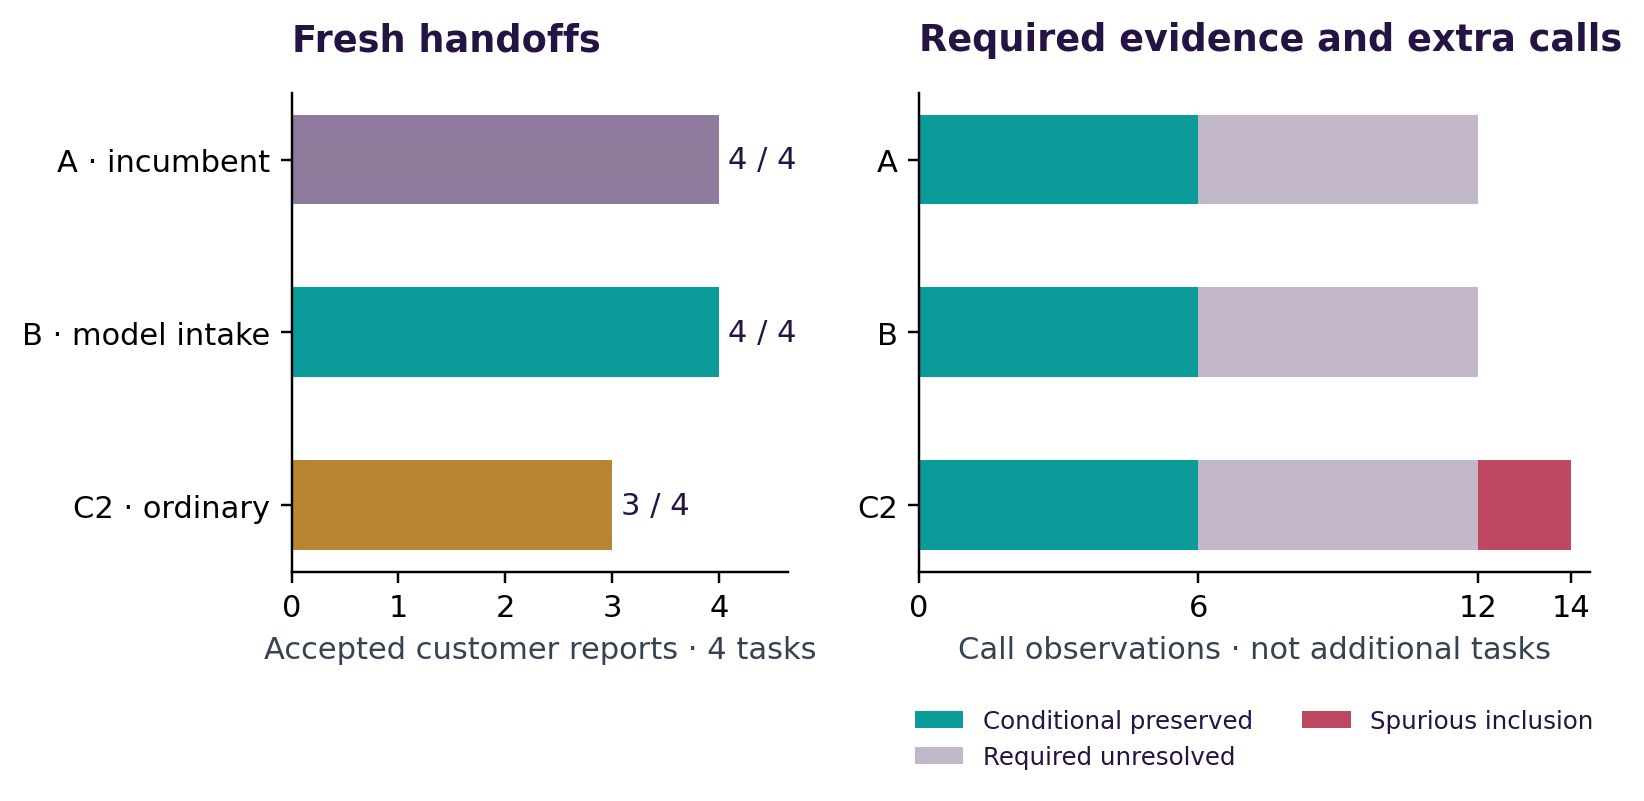
\includegraphics[width=\textwidth]{production-comparison.png}
\caption{Fresh customer-report acceptance and call-level evidence are different units. C2 covers the required calls but adds two out-of-scope data operations. The original failed primary remains a separate table and campaign.}
\end{figure}

The follow-up therefore demonstrates that prospective structured model intake can produce a source-bound customer review through the actual verifier. It does not identify a quality, operator-time or complete-cost gain over the incumbent. Its modest accuracy difference from this ordinary implementation is descriptive evidence on four purposive packages; it does not establish general superiority over competent conventional engineering.

A supplementary portability audit found a common integration defect outside the frozen customer-report checker: an auxiliary Workbench \texttt{fullTask} locator traversed one parent directory too few. All report links resolve and each exact raw task is attached, but the stronger claim that every original archive locator resolves is false for every arm. The sealed scores remain distinct from that finding. Publication assembly adds exact source aliases and records the repair separately without changing candidate code, output bytes or original acceptance. Complete source-license notices accompany the companion; standalone exports must retain the relevant notices.

The registered follow-up stopping rule is exhausted. C2 is not repaired against these answers, and the failed F03 task is not removed to create a favorable three-task cost comparison.
